\documentclass{article}

\usepackage{booktabs}
\usepackage[margin=1in]{geometry}
\usepackage{graphicx}
\usepackage{setspace}
\usepackage{threeparttable}

\newcommand{\mc}{\multicolumn}

\begin{document}

\noindent \large{\textbf{Parental Income in ABC/CARE}} \\

\doublespacing

Parental income is self-reported in the demographic and parent interviews. We are interested in earned income that excludes income from social programs or child support. Although it is not clear that earned income is what is being asked in the questionnaires, Margaret Burchinal advocates for treating the responses as earned income regardless. This is a plausible assumption given that there are other questions about alternate income sources that appear throughout the surveys. 

There are two ways earned income is reported: With categorical or continuous variables. In ABC, the categorical variables take 17 values ranging from no income (category 1) to greater than \$14,000 (category 16), including unknown income (category 17). The variables that take continuous values record the earned parental income that the respondent reports.

Using these measures of self-reported income, we calculate income in 2014 USD with the inflation rate matching the year of the interview. When the year of interview was missing, it was approximated using birthdate.

In ABC, there are some ages with only categorical variables (3.5 and 4.5 years). This presents an issue when comparing income at these ages with that at other ages for those individuals who earn at least \$14,000 in the dollars at the time of the interview. Figure~\ref{fig:pinc} shows the truncated data. To address this issue, we impute the income using the coefficients of the Tobit model of parental income on covariates that include income from years prior (standard errors are clustered at the individual level). This imputation was applied to those in ABC who indicated making \$14,000 or more when the child was 3.5 or 4.5 years old. This is an approximate solution that helps fill in missing values from the survey design. However, the imputed incomes are still low.

\begin{figure}
\centering
\caption{Parental Income before Imputation}\label{fig:pinc}
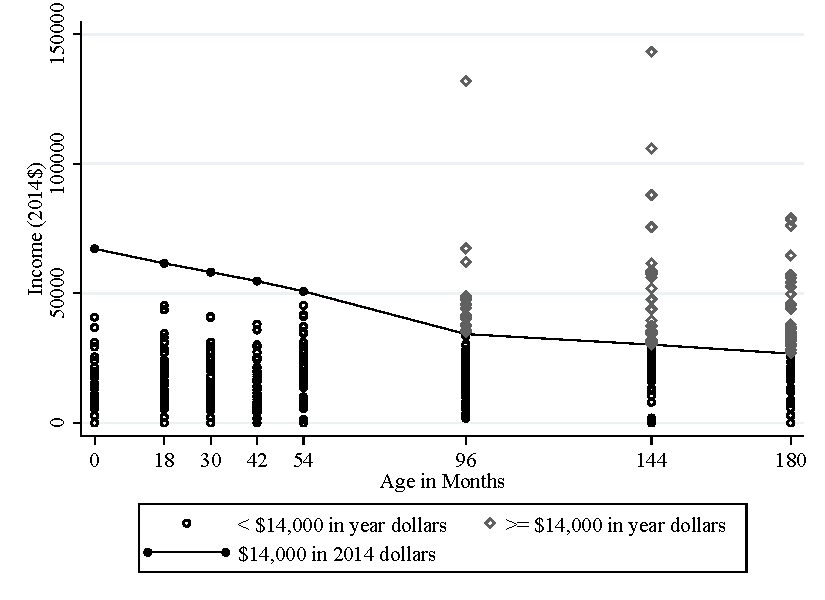
\includegraphics[width=\textwidth]{output/ABC-income-trunc}
\end{figure}


\end{document}